\chapter{Introducción y descripción del problema}

Este proyecto es software libre, y está liberado con la licencia \cite{gplv3}.


\section{Descripción general y motivación}

El término de Realidad Aumentada comprende al conjunto de técnicas y tecnologías que permiten la superposición e interacción de elementos virtuales sobre la realidad física a través de un dispositivo electrónico. Esta tecnología se ha aplicado a una gran variedad de ámbitos, tales como en la creación de filtros faciales para fotos en redes sociales como Instagram, dibujar la trayectoria que ha seguido el balón en la repetición de una jugada de fútbol, muestra de distintos gráficos y maquetas en los telediarios, previsualización de mobiliario en una habitación e incluso videojuegos como Pokemon GO.

El avance en las cámaras y procesadores de los teléfonos móviles en la última década ha facilitado que casi cualquier persona tenga en el bolsillo un dispositivo capaz de reproducir experiencias muy vistosas de Realidad Aumentada. Sin embargo en la mayoría de casos se trata de aplicaciones en las que el usuario consume pasivamente contenido pregenerado por los desarrolladores, sin la capacidad de crear ellos mismos estas experiencias.

Se propone entonces desarrollar en primer lugar una aplicación web que permita al usuario la composición de textit{escenas 3D} para uso en Realidad Aumentada (textit{RA} de aquí en adelante). Cuando hablamos de escena nos referimos una composición de uno o más modelos 3D con una disposición concreta. Por ejemplo podríamos colocar el modelo de un tobogán junto al de un columpio y un balancín, formando el conjunto la escena de un parque. La aplicación consistirá principalmente de un editor sencillo e intuitivo que permita cargar modelos 3D con texturas y aplicarles transformaciones para colocarlos en una escena. Adicionalmente se podrá añadir a la escena una pista de audio y reproducir animaciones de los modelos. Se podrá guardar la escena en un servidor web en una colección de escenas creadas asociadas a una cuenta de usuario, desde la cual se podrán modificar o eliminar.

Adicionalmente, el usuario podrá iniciar sesión en una app móvil Android para acceder a su lista de escenas creadas y podrá reproducir cualquiera de ellas en Realidad Aumentad con su dispositivo móvil.

Las principales motivaciones para elegir este como mi trabajo de fin de grado fue mi alto grado de interés por los gráficos 3D, mis conocimientos previos en tecnologías que acabaría usando como three.js o Android Studio, y que es un proyecto relativamente multidisciplinar, ya que requiere del desarrollo de una aplicación web, una aplicación Android y un servidor web que los conecte, creando así un pequeño ecosistema.

\section{Objetivos}

\section{Fundamentos}

\subsection{Realidad Aumentada}
\begin{figure}[h]
    \centering
    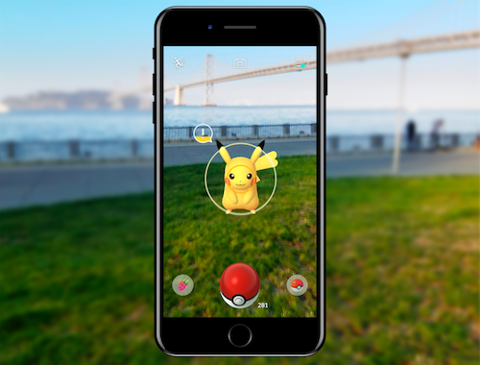
\includegraphics[scale=0.13]{pkmgo}
    \caption{Ejemplo de Realidad Aumentada en el videojuego Pokémon Go}
\end{figure}

\subsection{Metodologías de desarrollo ágil}

\subsection{Android}
\subsubsection{Android Studio}
\subsubsection{Kotlin}

\subsection{React}

\subsection{Typescript}

\subsection{Node.js}

\subsection{Express}

\subsection{Firebase}

\subsection{Sceneview}

\subsection{Archivo GLB}

